\chapter{Tesztelés és használat}
\label{ch:test}

A fejezet első fele a szerkesztő ellenőrzésének módját mutatja be, a második fele az elkészült alkalmazás használatát.

\section{Tesztelési stratégia}
\label{sec:test_strategy}

A tesztelés \aref{sec:architecture}. szakaszban leírt rétegeket követi. Minél lejjebb van egy kódrészlet a rétegek között, annál egyszerűbb és gyorsabb tesztelni, ezért a tesztek többsége az alsó rétegekre irányul. A geometriai számításokat, az útvonalak feldolgozását, a színértékek értelmezését, az SVG-importálást és -exportálást a tesztek közvetlenül, bemenetek és elvárt kimenetek alapján ellenőrzik.

Az eszközök tesztjei mesterséges \texttt{PointerInfo} eseményeket küldenek, majd a dokumentum és az előzmények állapotát vizsgálják. Egy téglalap rajzolásának tesztje például egy lenyomást, néhány mozgatást és egy felengedést ad át a téglalap eszköznek, és ellenőrzi, hogy pontosan egy új alakzat és egy új előzménybejegyzés keletkezett. A felület részeit, a vásznat, a paneleket, a színválasztót és a párbeszédablakokat, végül a teljes alkalmazást a tesztek a jsdom környezetében jelenítik meg~\cite{jsdom}, és DOM-eseményekkel kezelik.

A jsdom nem végez valódi elrendezést és megjelenítést, így például az elemek mérete és a szöveg szélessége nem mérhető vele. Ezeket a tesztek egyszerű közelítéssel helyettesítik, a valódi megjelenést pedig böngészőben ellenőriztem. Az automatikus teszteket valódi böngészőben végzett kézi tesztelés egészítette ki, és az ennek során talált hibákhoz a javítás előtt egy-egy automatikus teszt készült.

\section{Automatikus tesztek}
\label{sec:unit_tests}

A tesztek a Vitest keretrendszerrel futnak~\cite{vitest}, a \texttt{tests} mappában, témák szerint öt almappába rendezve. A tesztek témakörök szerinti megoszlása \aref{tab:tests}. táblázatban látható.

\begin{table}[!htbp]
\caption{Az automatikus tesztek elosztása}
\label{tab:tests}
\centering
\footnotesize
\begin{tabular}{|l|>{\raggedright\arraybackslash}p{0.52\textwidth}|r|r|}
\hline
\textbf{Mappa} & \textbf{Témakör} & \textbf{Fájl} & \textbf{Teszteset} \\ \hline
\texttt{model} & alakzatok, útvonalak, csoportok, színátmenetek, szaggatás, előzmények, projektfájl, beállítások, véletlenszerű tesztek & 12 & 114 \\ \hline
\texttt{tools} & rajzolás, kijelölés, csomópontok, illesztés, logikai műveletek, olló, foltecset & 7 & 71 \\ \hline
\texttt{io} & SVG-importálás és -exportálás, raszteres export, képek, vágólap & 6 & 64 \\ \hline
\texttt{fonts} & Google Fonts kérések, helyi betűtípusok, beágyazás, szöveg útvonallá alakítása, betűtípus-választó & 7 & 79 \\ \hline
\texttt{ui} & vászon, panelek, színválasztó, párbeszédablakok, nézet, teljes alkalmazás, regressziós tesztek & 8 & 81 \\ \hline
\textbf{Összesen} & & \textbf{40} & \textbf{409} \\ \hline
\end{tabular}
\end{table}

A forráskódban 409 teszteset szerepel. Futtatáskor a keretrendszer 447 tesztet jelez, mert a véletlenszerű tesztek egyik tesztesete negyven különböző kezdőértékkel fut le. A teljes tesztkészlet egy átlagos fejlesztői gépen 30-40 másodperc alatt fut le, és minden módosítás után könnyen lefuttatható. \Aref{tab:req-tests}. táblázat azt mutatja, mely tesztfájlok ellenőrzik \aref{tab:requirements}. táblázat követelményeit.

\begin{table}[!htbp]
\caption{A funkcionális követelmények és az őket ellenőrző tesztfájlok}
\label{tab:req-tests}
\centering
\footnotesize
\renewcommand{\arraystretch}{1.15}
\begin{tabular}{|l|>{\raggedright\arraybackslash}p{0.2\textwidth}|>{\raggedright\arraybackslash}p{0.6\textwidth}|}
\hline
\textbf{Az.} & \textbf{Terület} & \textbf{Tesztfájlok} \\ \hline
F1 & Elrendezés & \texttt{ui/app}, \texttt{ui/panels}, böngészős ellenőrzés \\ \hline
F2 & Rajzolás & \texttt{tools/drawing}, \texttt{ui/canvas} \\ \hline
F3 & Tulajdonságok & \texttt{model/shapes}, \texttt{tools/select}, \texttt{ui/panels} \\ \hline
F5 & Szöveg & \texttt{fonts/text}, \texttt{fonts/outline}, \texttt{fonts/textOutline}, \texttt{ui/canvas} \\ \hline
F6 & Színek & \texttt{model/gradient}, \texttt{model/dash}, \texttt{ui/color-picker} \\ \hline
F7 & Útvonalak & \texttt{model/path}, \texttt{model/strokeToPath}, \texttt{tools/edit}, \texttt{tools/boolean}, \texttt{tools/scissors} \\ \hline
F8 & Illesztés, igazítás & \texttt{tools/snap} \\ \hline
F9 & Objektumok & \texttt{model/groups}, \texttt{model/lock} \\ \hline
F10 & Kijelölés & \texttt{tools/select}, \texttt{ui/canvas-tools} \\ \hline
F11 & Vágólap & \texttt{io/clipboard} \\ \hline
F12 & Nagyítás & \texttt{ui/view}, böngészős ellenőrzés \\ \hline
F13 & Visszavonás & \texttt{model/history}, \texttt{model/fuzz} \\ \hline
F14 & Mentés & \texttt{model/project}, \texttt{model/preferences} \\ \hline
F15 & Import, export & \texttt{io/import}, \texttt{io/serializer}, \texttt{io/export}, \texttt{io/images}, \texttt{fonts/embed} \\ \hline
\end{tabular}
\end{table}

\newpage

Néhány jellemző eset a tesztek közül:

\begin{itemize}
\item egy elforgatott téglalap importálás után elforgatott téglalap marad, egy nyírt téglalap viszont útvonallá alakul;
\item egy csoport exportálás és újbóli importálás után is megtartja a forgatását és az átlátszóságát;
\item két kör egyesítése néhány görbe csomópontot ad, nem sokszöget;
\item a szöveg útvonallá alakításakor az ,,o'' betű két kontúrt kap, egy külsőt és egy belső lyukat, a magyar ,,ő'' és ,,ű'' betű pedig helyesen jelenik meg;
\item egy ismeretlen betűtípusú szöveget a szerkesztő nem alakít útvonallá, a szöveg szöveg marad.
\end{itemize}

\section{Véletlenszerű tesztelés}
\label{sec:fuzz}

A kézzel írt tesztek azokat az eseteket ellenőrzik, amelyekre a fejlesztő gondolt. A szerkesztőben viszont a műveletek tetszőleges sorrendben követhetik egymást, és egyes hibák csak ritka kombinációkban jelentkeznek, például egy csoportba belépve, egy forgatás és egy visszavonás után. Ezek felderítésére véletlenszerű műveletsorozatokat végrehajtó teszt készült, angol nevén \textit{fuzzing}. A módszer Miller és társai 1990-es vizsgálatából ered, amelyben véletlenszerű bemenettel a UNIX-segédprogramok negyedét-harmadát sikerült összeomlasztani~\cite{miller1990}.

A teszt egy kezdőértékkel inicializált álvéletlenszám-generátor alapján súlyozottan választ a műveletek közül. Alakzatokat rajzol az eszközökkel, mozgat, méretez, forgat, csoportosít, csoportba lép be, csomópontokat szerkeszt, stílust módosít, visszavon és megismétel. Az ellenőrzés a QuickCheck eszközzel ismertté vált tulajdonságalapú tesztelést követi~\cite{claessen2000}, vagyis nem egy konkrét kimenetet vár, hanem olyan állításokat, amelyeknek minden állapotban igaznak kell lenniük. Minden lépés után néhány olcsón ellenőrizhető tulajdonságot vizsgál, például hogy a kijelölés pontosan a belépett csoport szintjén lévő alakzatokra vonatkozik. Néhány lépésenként és a futás végén költségesebb ellenőrzések is lefutnak:

\begin{itemize}
\item a projektfájlba mentett, majd visszatöltött dokumentum ugyanazokat az alakzatokat adja ugyanott
\item az exportált SVG minden útvonal csomópontjait tartalmazza
\item az összes lépés visszavonása után a kiinduló dokumentum áll vissza
\end{itemize}

Alapértelmezés szerint negyven kezdőérték fut le, egyenként százötven lépéssel, és egy további futás hétszáz lépéssel, amely túllépi az előzmények kétszáz lépéses korlátját. Hiba esetén a teszt kiírja a kezdőértéket és az utolsó műveleteket, a hibás sorozat tehát pontosan megismételhető.

\section{Betűtípusok tesztelése hálózat nélkül}
\label{sec:fake_google}

A betűtípusokkal kapcsolatos kód nagy része a Google Fonts és a Fontsource szolgáltatásainak küld kéréseket. A tesztek nem használhatják a valódi hálózatot, mert akkor lassúak és megbízhatatlanok lennének. Egy segédmodul ezért helyettesíti a szolgáltatásokat, és ott, ahol ez számít, a valódi API viselkedését utánozza. Egy nem létező stílus kérését az egész kérés elutasításával válaszolja meg, a \texttt{text} paraméteres kérésre egyetlen \texttt{@font-face} blokkot ad, a paraméter nélküli kérésre pedig írásrendszerenként egyet~\cite{google-fonts-css2}. Betűtípusfájlként a tesztkészletben tárolt kis betűtípusfájlokat küldi vissza.

\section{Kézi tesztelés és regressziós tesztek}
\label{sec:manual_tests}

A kézi tesztelés során a felület minden részét végigpróbáltam, és a talált hibákat egy hibalistába gyűjtöttem. A hibák egy része csak a komponensek együttműködésében jelentkezett, ezért a hozzájuk tartozó tesztek a teljes vásznat jelenítik meg. \Aref{tab:regressions}. táblázat a hibalista néhány jellemző bejegyzését és a hozzájuk tartozó teszteket mutatja. A tesztek neve a hiba azonosítójával kezdődik, egy hiba újbóli megjelenése tehát azonnal azonosítható.

\begin{table}[!htbp]
\caption{Hibák a kézi tesztelésből és a hozzájuk tartozó regressziós tesztek}
\label{tab:regressions}
\centering
\footnotesize
\begin{tabular}{|l|>{\raggedright\arraybackslash}p{0.78\textwidth}|}
\hline
\textbf{Azonosító} & \textbf{A teszt által ellenőrzött viselkedés} \\ \hline
B-01 & Az exportált SVG jól formált XML, és nem függ külső betűtípustól. \\ \hline
B-02 & Egy csomópont húzása közben a csomópontok és a fogantyúk a görbével együtt mozognak. \\ \hline
B-03 & A toll eszközzel az első pontra lenyomva és húzva kattintásként viselkedik, a későbbi pontok viszont sima csomóponttá húzhatók. \\ \hline
B-04 & Az útvonal bezárásának előnézete pontosan azt az alakzatot mutatja, amelyet a kattintás létrehoz. \\ \hline
B-05 & Rajzolás és kijelölés után a mozgatás, a méretezés és a forgatás a kijelölő keretet is mozgatja. \\ \hline
B-06 & A kijelölés megszüntetése, legyen az kattintás az üres vászonra, Esc vagy dupla kattintás, eltünteti a kijelölő keretet. \\ \hline
\end{tabular}
\end{table}

\section{Böngészős ellenőrzés és a kész alkalmazás mérete}
\label{sec:browser_check}

A fejlesztés során az alkalmazást folyamatosan egy Chromium-alapú asztali böngészőben használtam, a kézi tesztelés is ott történt. A jsdom által nem vizsgálható viselkedés, például a valódi elrendezés, a szöveg mérése, a raszteres export és az érintéses mozdulatok ellenőrzésének egy részét a Playwright eszközzel szkriptekbe foglaltam~\cite{playwright}. A Playwright programból vezérel egy Chromium böngészőt, asztali és telefonos képernyőméretre is beállítható, és érintéses eseményeket is küldhet. A dolgozat képernyőképei is így készültek. A felületet Firefox böngészőben is kipróbáltam, ott is helyesen működik, Safari böngészőben azonban nem teszteltem. A helyi betűtípusok elérése a Chromium-alapú böngészőkre korlátozódik, ezt \aref{sec:text_impl}. szakasz tárgyalja.

Az éles változatot a Vite csomagolja. A keletkező fő JavaScript-fájlokat \aref{tab:bundle}. táblázat sorolja fel. A nagy könyvtárak dinamikus importtal külön fájlba kerülnek, és csak az első használatukkor töltődnek be: a paper.js az első logikai műveletnél vagy vágásnál, a fontkit és a WOFF2 kibontó az első útvonallá alakításnál. Az alkalmazás indulásakor ezért csak a fő fájlt kell letölteni, amely tömörítve körülbelül 160 kB.

\begin{table}[!htbp]
\caption{Az éles változat fő JavaScript-fájljai}
\label{tab:bundle}
\centering
\footnotesize
\begin{tabular}{|l|l|r|r|}
\hline
\textbf{Fájl} & \textbf{Tartalom} & \textbf{Méret} & \textbf{Tömörítve} \\ \hline
\texttt{index} & a szerkesztő kódja & 504,2 kB & 160,8 kB \\ \hline
\texttt{paper-core} & paper.js & 318,9 kB & 112,3 kB \\ \hline
\texttt{browser-module} & fontkit & 363,0 kB & 150,5 kB \\ \hline
\texttt{decompress} & WOFF2 kibontó & 295,2 kB & 127,0 kB \\ \hline
\end{tabular}
\end{table}

\section{Az alkalmazás használata}
\label{sec:usage}

Indításkor az alkalmazás a legutóbbi automatikus mentést tölti vissza, ennek hiányában üres lappal nyílik meg. \Aref{fig:ui-main}. ábra a szerkesztőt asztali képernyőn mutatja. A rajzon egy kijelölt kör látható a nyolc méretező fogantyúval, a felette lévő forgató fogantyúval és a közepén a forgatási középponttal. A jobb oldali kitöltés panelen a kör sugárirányú színátmenete szerkeszthető. A színátmenet sávja alatt a színpontok, alattuk a színválasztó, legalul pedig az átmenet középpontja és sugara látható.

\begin{figure}[!htbp]
\centering
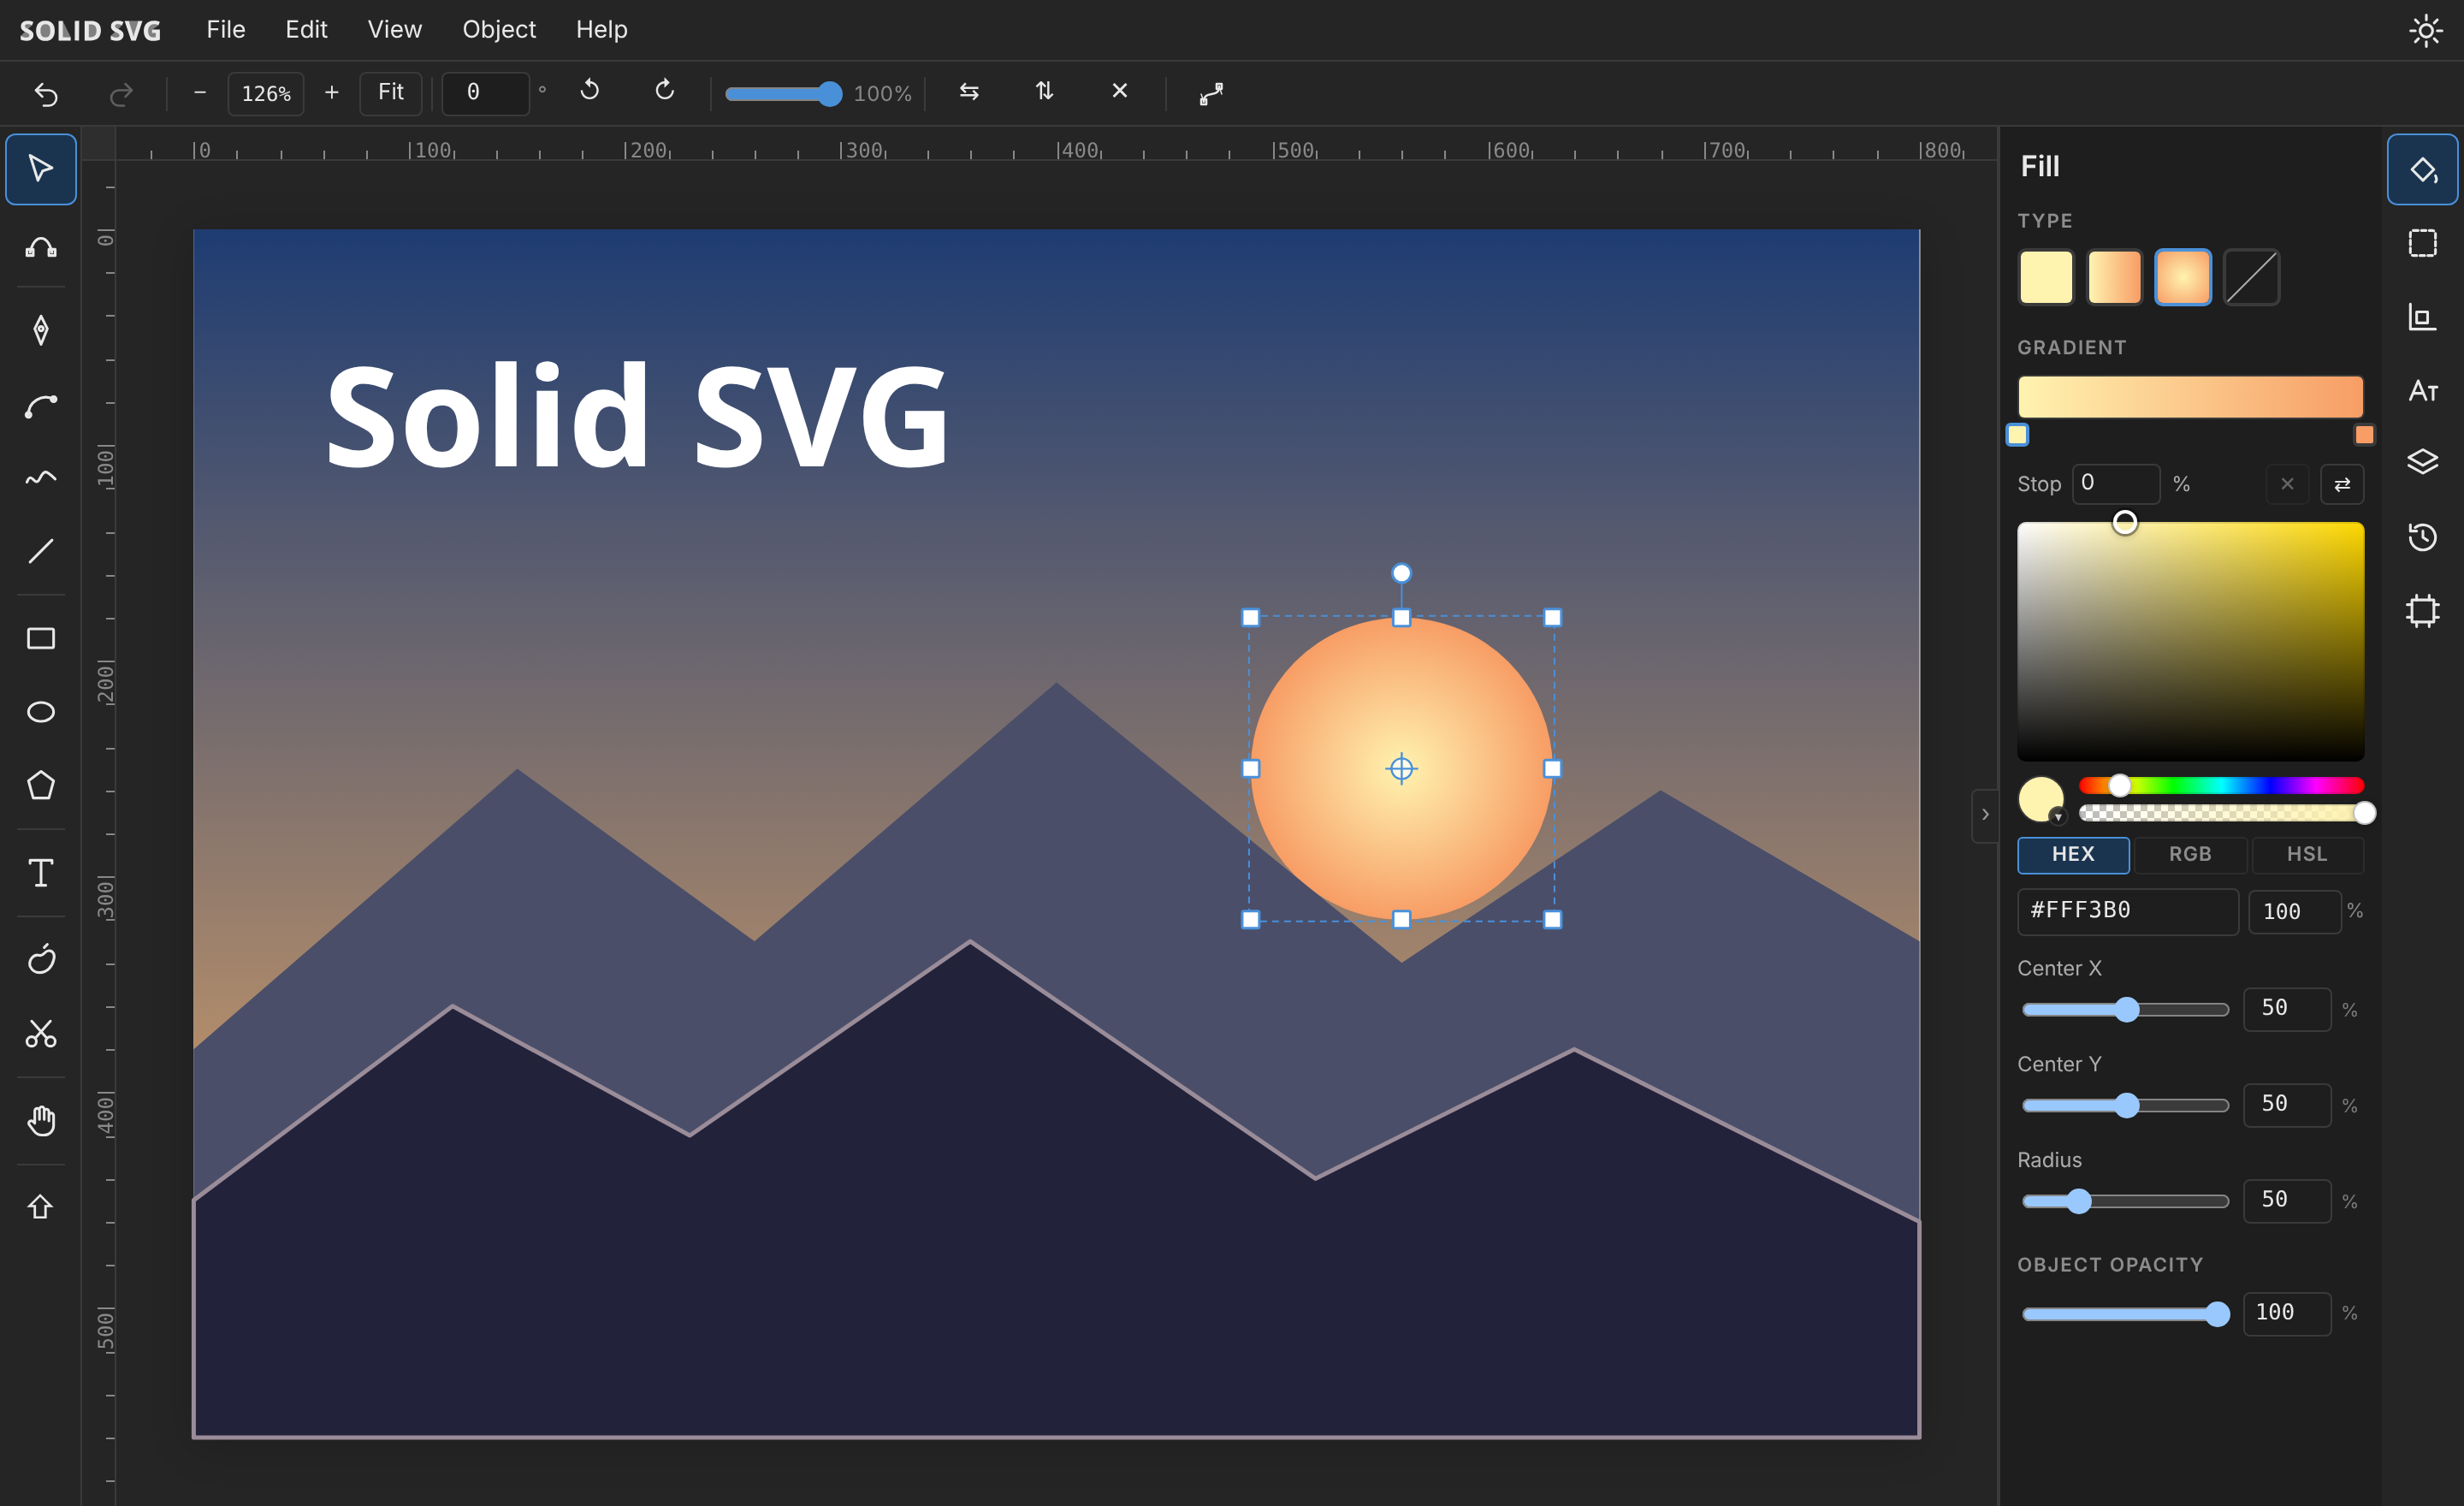
\includegraphics[width=\textwidth]{images/editor/ui-main.png}
\caption{A szerkesztő felülete asztali képernyőn, egy kijelölt alakzattal és a kitöltés panellel}
\label{fig:ui-main}
\end{figure}

\paragraph{Rajzolás.} Az eszköz a bal oldali eszköztárról vagy a billentyűjével választható ki. A téglalap, az ellipszis és a vonal húzással rajzolható, Shift billentyűvel négyzet, kör, illetve 45 fokos lépésekben elforgatott vonal készül. A sokszög eszköz kattintásonként egy csúcsot ad hozzá, a toll és a körív \aref{sec:drawing_tools}. szakaszban leírtak szerint működik. A szöveg eszközzel a vászonra kattintva közvetlenül lehet gépelni. Az eszközök billentyűit \aref{tab:tool-keys}. táblázat foglalja össze.

\begin{table}[!htbp]
\caption{Az eszközök és billentyűik}
\label{tab:tool-keys}
\centering
\footnotesize
\begin{tabular}{|l|c||l|c||l|c|}
\hline
\textbf{Eszköz} & \textbf{Bill.} & \textbf{Eszköz} & \textbf{Bill.} & \textbf{Eszköz} & \textbf{Bill.} \\ \hline
Kijelölés & V & Szabadkézi rajz & F & Szöveg & T \\ \hline
Csomóponteszköz & E & Vonal & L & Foltecset & Shift+B \\ \hline
Toll & B & Téglalap & R & Olló & C \\ \hline
Körív & A & Ellipszis & O & Nézet mozgatása & H \\ \hline
 & & Sokszög & P & & \\ \hline
\end{tabular}
\end{table}

\paragraph{Objektumok és geometria.} Az objektumok panel, a felületen \textit{Objects}, a dokumentum fáját mutatja, ez látható \aref{fig:panels}. ábra bal oldalán. Minden sorban ott van az alakzat típusának ikonja, a neve és a kitöltése, a kijelölt sorban pedig a zárolás és az elrejtés gombja is. A sorok húzással rendezhetők, és egy sort egy csoportra húzva az alakzat a csoportba kerül. Az ábra közepén a geometria panel, a felületen \textit{Geometry}, a pozíciót, a méretet, a forgatási középpontot és a forgatást mutatja. A forgatási középpont a határoló téglalap százalékában vagy a mellette lévő kilenc pont egyikével adható meg. Az ábrán a bal alsó sarokba került, a kijelölt hegyek tehát a bal alsó sarkuk körül fordulnának el.

\begin{figure}[!htbp]
\centering
\begin{minipage}[b]{0.31\textwidth}\centering
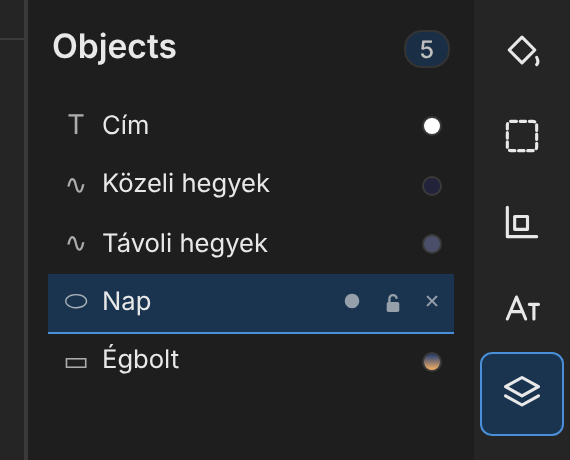
\includegraphics[width=\textwidth]{images/editor/ui-objects.png}\\[2pt]
{\footnotesize Objektumok panel}
\end{minipage}\hfill
\begin{minipage}[b]{0.31\textwidth}\centering
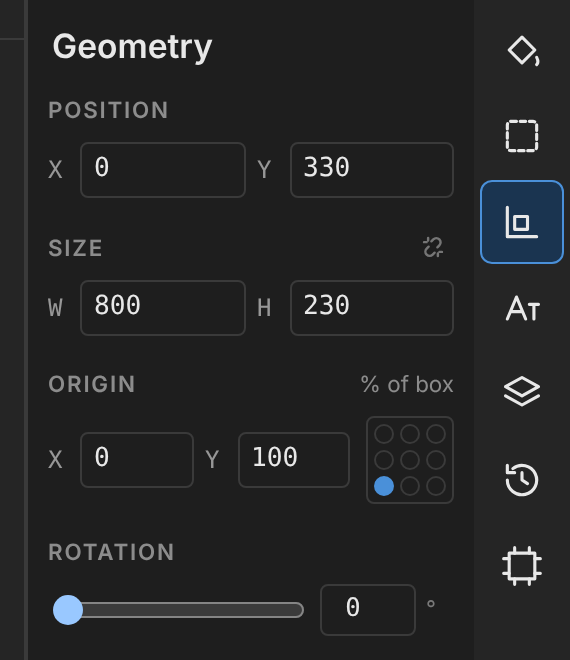
\includegraphics[width=\textwidth]{images/editor/ui-geometry.png}\\[2pt]
{\footnotesize Geometria panel}
\end{minipage}\hfill
\begin{minipage}[b]{0.33\textwidth}\centering
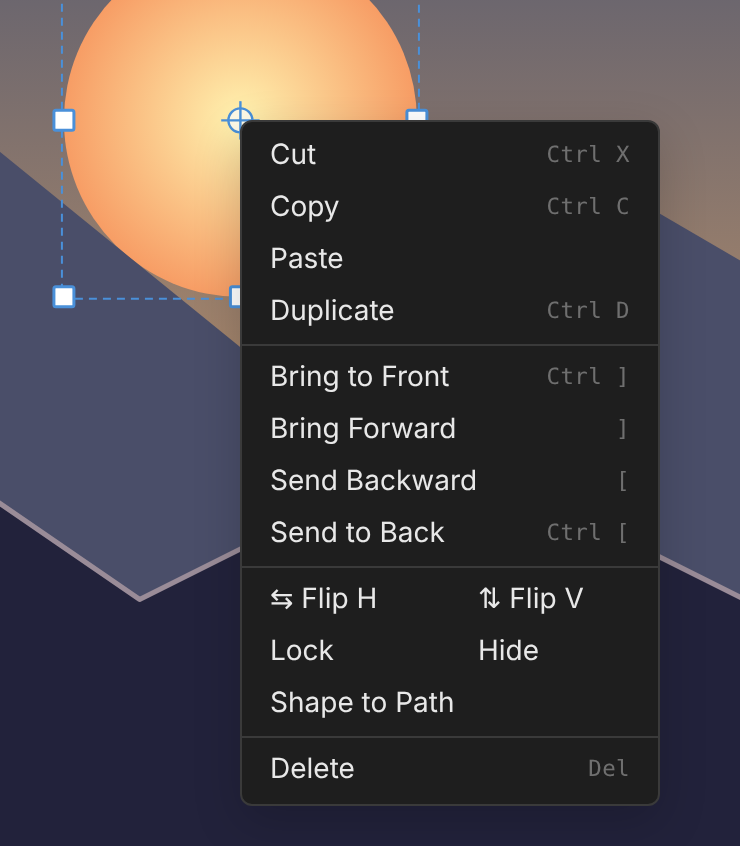
\includegraphics[width=\textwidth]{images/editor/ui-context-menu.png}\\[2pt]
{\footnotesize Helyi menü}
\end{minipage}
\caption{Az objektumok panel, a geometria panel és egy alakzat helyi menüje}
\label{fig:panels}
\end{figure}

\paragraph{Helyi menü.} Egy alakzatra jobb egérgombbal kattintva vagy érintőképernyőn hosszan megérintve megjelenik a helyi menü, \aref{fig:panels}. ábra jobb oldalán. A menüben csak az adott helyzetben elérhető műveletek szerepelnek: a vágólap műveletei, a sorrend módosítása, a tükrözés, a zárolás, az elrejtés, az útvonallá alakítás és a törlés. A billentyűkombinációk a menüpontok mellett is láthatók.

\paragraph{Mentés és exportálás.} A \textit{File} menü kínálja az új dokumentumot, a projekt vagy SVG-fájl megnyitását, a projekt mentését, SVG-fájlok és képek beillesztését a meglévő rajzba, valamint az exportálást SVG és raszteres formátumba. Az exportálás beállításai külön párbeszédablakban adhatók meg, amelyet \aref{fig:export}. ábra mutat. Itt választható ki, hogy a lap vagy csak a rajzolt alakzatok környezete kerüljön a fájlba, hogy a háttér is része legyen-e, és hogy a szöveg \aref{sec:svg_io}. szakaszban leírt módok közül melyikkel hagyja el a szerkesztőt. A raszteres képek mérete és minősége is itt állítható.

\paragraph{Telefonon.} Keskeny kijelzőn a felület \aref{fig:mobile}. ábrán látható módon rendeződik át. A tulajdonságpanel a vászon alatt jelenik meg, az eszköztár és a tulajdonságsáv a két oldalon marad. Az eszköztár alján lévő nyíl gomb a Shift billentyűt helyettesíti, bekapcsolva például a téglalap eszköz négyzetet rajzol, és a kijelölés bővíthető. A nézet két ujjal nagyítható és mozgatható.

{\restylefloat*{figure}
\begin{figure}[!htbp]
\centering
\begin{minipage}[b]{0.46\textwidth}\centering
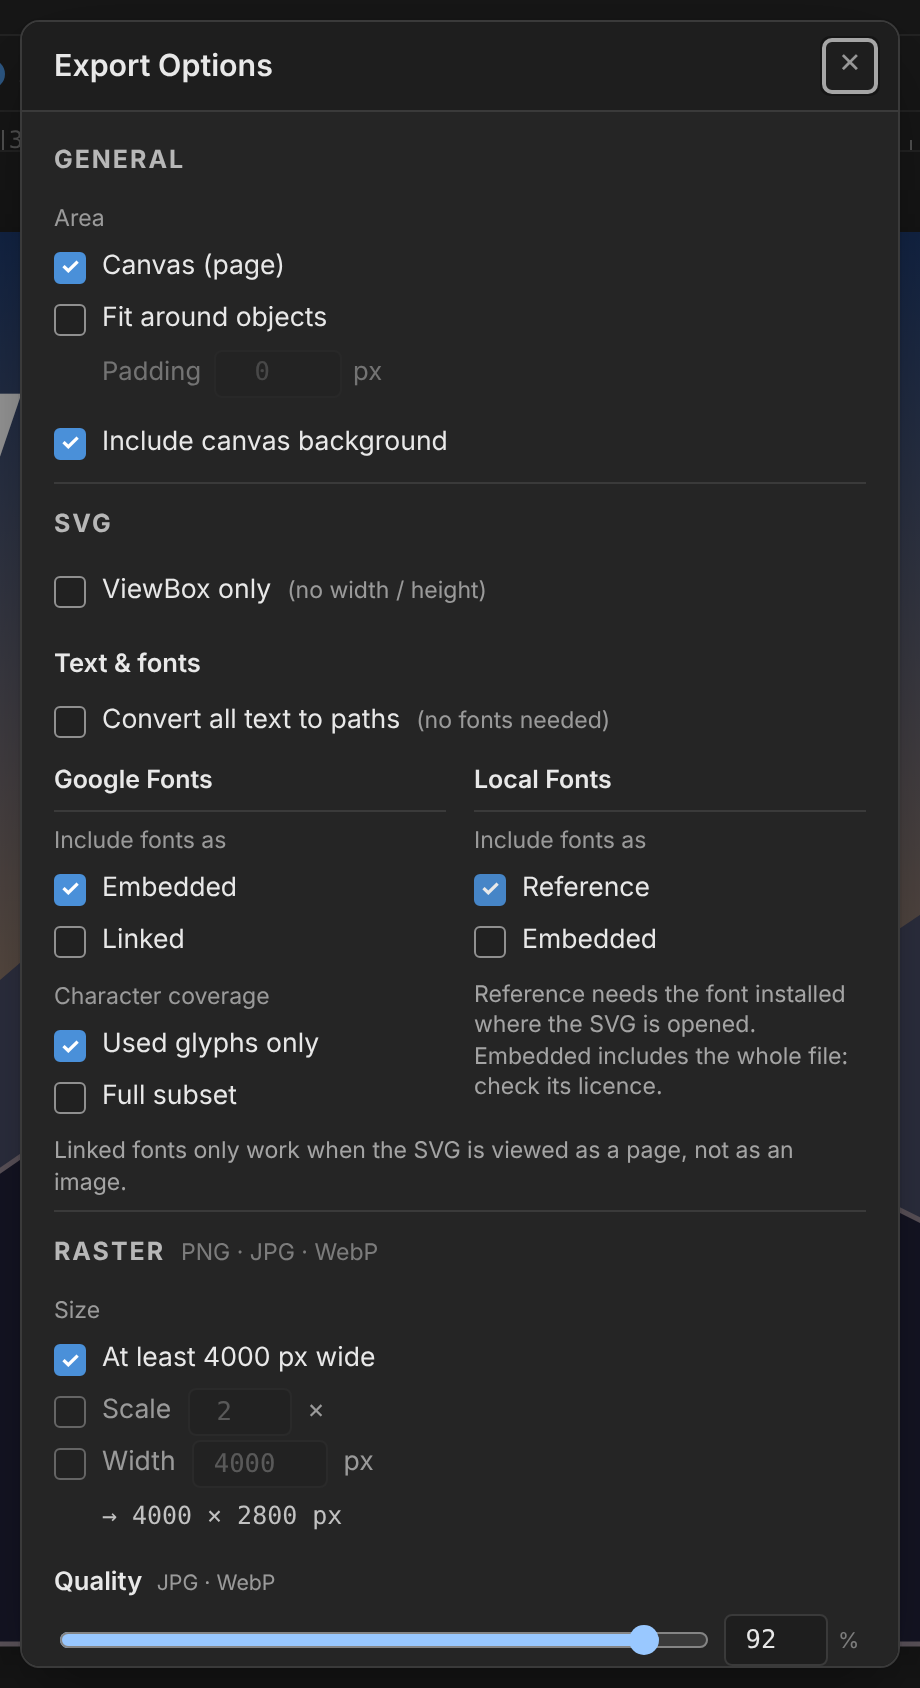
\includegraphics[height=0.5\textheight]{images/editor/ui-export.png}
\caption{Az exportálási beállítások párbeszédablakja}
\label{fig:export}
\end{minipage}\hfill
\begin{minipage}[b]{0.46\textwidth}\centering
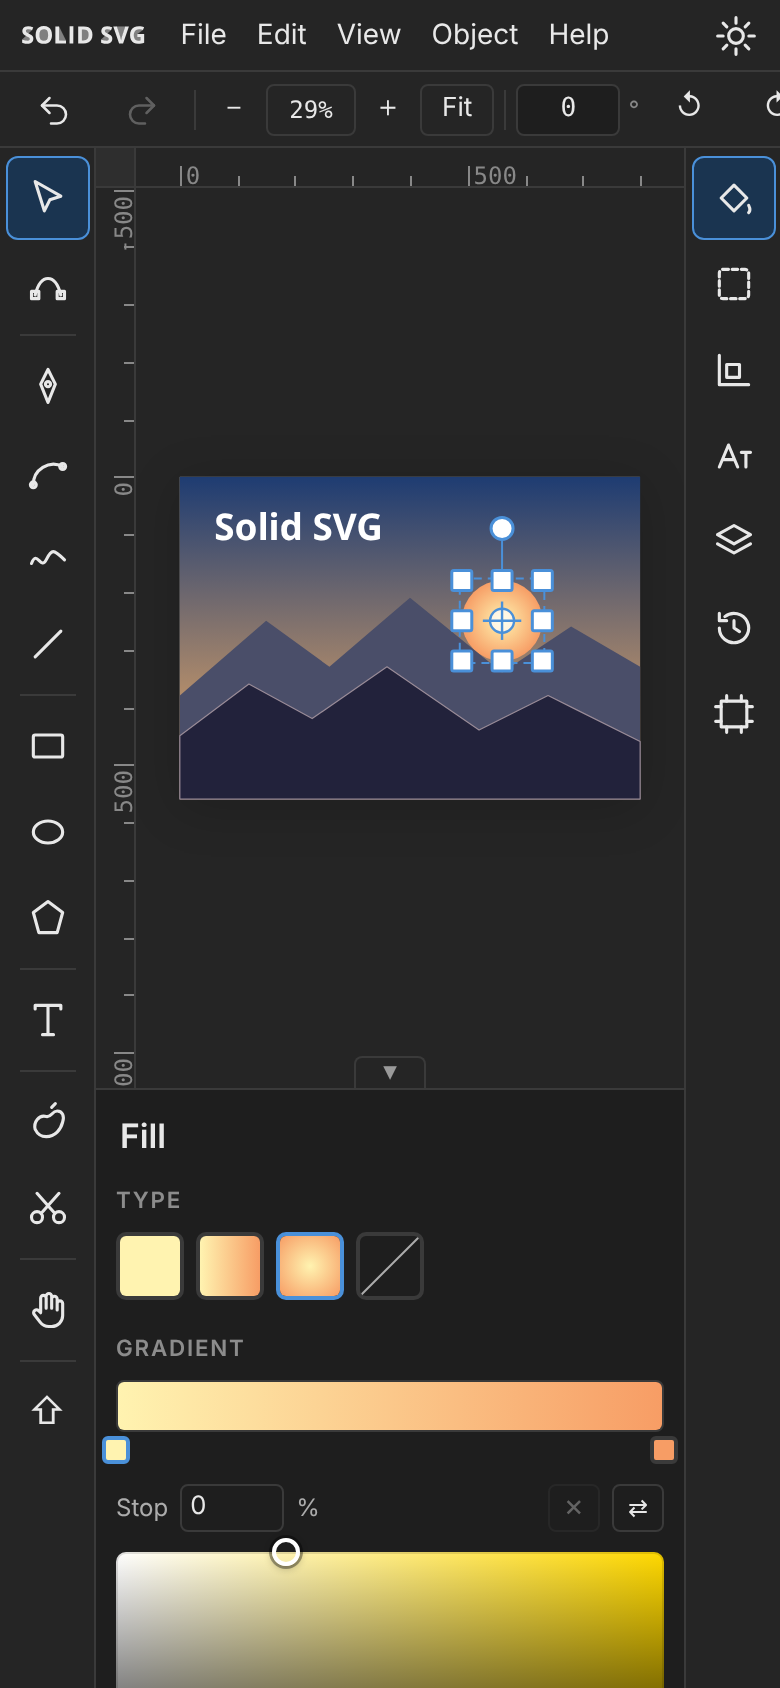
\includegraphics[height=0.5\textheight]{images/editor/ui-mobile.png}
\caption{A szerkesztő telefonon, nyitott tulajdonságpanellel}
\label{fig:mobile}
\end{minipage}
\end{figure}  
}